% !TEX program = xelatex
%!TEX encoding = UTF-8 Unicode
%%%%%%%%%%%%%%%%%%%%%%%%%%%%%%%%%%%%%%%%%%%%%%%%%%%%%%%%%%%%%%%%%%%%%%%%%%%%%%%%%%%
%%
%%
%%
%% Copyright (C) 2016, Lingxiao Zhao. 赵令霄
%% Department of Electrical Engineering, Xi'an Jiaotong University.
%% Email: lingxia1@andrew.cmu.edu
%% Version 1.1 
%%
%% Made a huge improvement accoding to the word template provided by XJTU!!!
%%%%%%%%%%%%%%%%%%%%%%%%%%%%%%%%%%%%%%%%%%%%%%%%%%%%%%%%%%%%%%%%%%%%%%%%%%%%%%%%%%%
%Reference: 
% 1.  NJU Latex Model from Chuheng Zhang
%% 作者:张楚珩,zhangchuheng123 (at) live (dot) com
%% 个人主页: http://sealzhang.tk
%% 感谢Hu Haixing提供的南京大学硕博学位论文模板
%% 项目主页:http://haixing-hu.github.io/nju-thesis/
%%
% 2. XJTU CTex Model from 
%  MCMTHESIS.cls  CopyLeft 2011/8/24 by
%  wanghongxin <hongxin_w@163.com>
%  hugo <>
%  hy_haoyun <haoyun_tex@163.com>
%%%%%%%%%%%%%%%%%%%%%%%%%%%%%%%%%%%%%%%%%%%%%%%%%%%%%%%%%%%%%%%%%%%%%%%%%%%%%%%%%%%
% 使用说明:
% 1.首先在下面[Mac]处自行改系统
% 2.第二个section给出了常用功能用法示范
%====================================%
% 3.中文文献在生成Bibtex的时候加入:language ={zh},如:
% @article{陈润泽2014含储热光热电站的电网调度模型与并网效益分析,
%   title={含储热光热电站的电网调度模型与并网效益分析},
%   author={陈润泽 and 孙宏斌 and 李正烁 and 刘一兵},
%   journal={电力系统自动化},
%   volume={19},
%   pages={001},
%   year={2014},
%   language ={zh}    % 加入这一行
% }
%====================================%
% 4.当很多公式连续在一起时,采用\begin{gather}或\begin{align}环境替换\begin{gather},具体用法google
%                        
%%%%%%%%%%%%%%%%%%%%%%%%%%%%%%%%%%%%%%%%%%%%%%%%%%%%%%%%%%%%%%%%%%%%%%%%%%%%%%%%%%%
\documentclass[Win]{xjtuBSThesis}  % 输入Mac or Linux or Win 
%%%%%%%%%%%%%%%%%%%%%%%%%%%%%%%%%%%%%用户使用处%%%%%%%%%%%%%%%%%%%%%%%%%%%%%%%%%%%%%%%%%%%%%%%%%%
% 以下三项是必须的。
\let\cleardoublepage\clearpage
\author{刘志宏}{Zhihong Liu} % 作者{中文}{英文}
\title{基于二维Shapley Value的数据定价}{Value Evaluation Based on Two Dimensional Shapley Value}  % 题目{中文}{英文}
\advisor{常象宇}{Xiangyu Chang}  % 导师{中文}{英文}
%\date{}                                           % Activate to display a given date or no date
\usepackage{listings}
\usepackage{ctex}
\lstset{
	basicstyle          =   \footnotesize,          % 基本代码风格
	keywordstyle        =   \bfseries,          % 关键字风格
	commentstyle        =   \rmfamily\itshape,  % 注释的风格,斜体
	stringstyle         =   \ttfamily,  % 字符串风格
	flexiblecolumns,                % 别问为什么,加上这个
	numbers             =   left,   % 行号的位置在左边
	showspaces          =   false,  % 是否显示空格,显示了有点乱,所以不现实了
	numberstyle         =   \zihao{-5}\ttfamily,    % 行号的样式,小五号,tt等宽字体
	showstringspaces    =   false,
	captionpos          =   t,      % 这段代码的名字所呈现的位置,t指的是top上面
	frame               =   lrtb,   % 显示边框
}

\lstdefinestyle{Python}{
	language        =   Python, % 语言选Python
	basicstyle      =   \zihao{-5}\ttfamily,
	numberstyle     =   \zihao{-5}\ttfamily,
	keywordstyle    =   \color{blue},
	keywordstyle    =   [2] \color{teal},
	stringstyle     =   \color{magenta},
	commentstyle    =   \color{red}\ttfamily,
	breaklines      =   true,   % 自动换行,建议不要写太长的行
	columns         =   fixed,  % 如果不加这一句,字间距就不固定,很丑,必须加
	basewidth       =   0.5em,
}
\begin{document}

\includepdf[pages={1,2,3,4}]{model}  % 用于导入前几页任务书和评审表。

\frontmatter
\let\cleardoublepage\clearpage
\begin{abstractcn} % 中文摘要

继农业经济时代的劳动、土地,工业经济时代的资本、技术后,数据已成为数字经济时代的关键生产要素,党的十九届四中全会也首次将数据增列为一种生产要素。据《2021年中国数字经济发展白皮书》显示,2020年数字经济的市场规模已达39.2万亿元,占GDP的38.6\%,数字经济蓬勃发展对数据要素市场化配置提出更强烈需求。本文基于数据交易市场可能出现的一种情形进行数据定价,即在各方提供自己数据的背景下(假设是样本-特征类型的数据结构),依托数据训练出的模型所带来的经济效益应该如何公平合理地分配。上述问题也是一个按照样本与特征分配价值的二维问题。本文在假设数据完整与不考虑标签标注的前提下,利用Shapley value公平的价值分配机制,将一维情景下的数据定价问题推广到二维情景,从互动与公理化两个角度证明,并得到二维情形下的Shapley value公式及其唯一性。接下来将公式期望化并利用Monte-Carlo方法计算,最后利用实验检验上述计算方法的收敛性与可行性,最终证实二维场景下的Shapley value在上述背景下是正确的。


\end{abstractcn}

\keywordscn{数据定价;生产要素;Shapley value;二维} % 中文关键词
\let\cleardoublepage\clearpage
\begin{abstracten} % 英文摘要



Following labor and land in the agricultural economy era, and capital and technology in the industrial economy era, data has become a key production factor in the digital economy era. The Fourth Plenary Session of the 19th Central Committee of the Communist Party of China also added data as a production factor for the first time. According to the "White Paper on the Development of China's Digital Economy in 2021", the market size of the digital economy will reach 39.2 trillion yuan by 2020, accounting for 38.6\% of GDP. The vigorous development of the digital economy has put forward a stronger demand for the market-based allocation of data elements. In this paper, data pricing is based on a situation that may occur in the data trading market, that is, in the context of each party providing their own data (assuming a data structure of sample-feature type), the economic benefits brought by the model trained on the data should be How to distribute fairly and equitably. The above problem is also a two-dimensional problem of assigning values ​​according to samples and features. Under the premise of assuming complete data and not considering labels, this paper uses the fair value distribution mechanism of Shapley value to generalize the data pricing problem in one-dimensional scenarios to two-dimensional scenarios, proves it from the perspectives of interaction and axiomatic, and obtains Shapley value formula and its uniqueness in two-dimensional case. Next, the formula is expected and calculated by the Monte-Carlo method. Finally, the convergence and feasibility of the above calculation method are tested by experiments, and it is finally confirmed that the Shapley value in the two-dimensional scene is correct in the above context.



\end{abstracten}

\keywordsen{Value evaluation; Production factor; Shapley value; Two dimension } % 英文关键词
\let\cleardoublepage\clearpage
\tableofcontents % 生成目录

%================================================
%	正文
%================================================
\mainmatter
\let\cleardoublepage\clearpage
\section{绪论}
随着机器学习技术与人工智能算法的深入发展,数据带来的战略性意义愈发显著。为了训练出良好的模型,我们总是需要大量而且优质的数据。在现实场景下,训练所需要的数据往往分散在不同的机构或者组织当中,因此我们需要一个数据交易的平台,来实现多方数据的汇聚与合作,即“数据市场”,并借此产生经济价值和社会效益。在这种场景下,数据显然成为了不可忽视的生产要素。宏观经济学强调,经济的发展离不开劳动力、土地、资本和企业家才能等生产要素的推动\cite[66]{赵英军2004西方经济学}。党的十九届四中全会首次将数据增列为一种生产要素,要求建立健全由市场评价贡献、按贡献决定报酬的机制。具体来说,就是需要建立一套公平合理的数据
市场交易体系。而在要素市场中,要素在价值生产中的贡献值不可直接测定,只能通过市场经济的竞争简化为要素价格信号,数据定价机制的建立是完善数据市场生态体系的关键问题。目前,产业领域存在两种较为普遍的数据定价机制:一是互联网服务商等推出的以自身为主的数据服务平台或产品,如谷歌云平台采取每分钟计价模式和持续折扣模式。二是数据交易平台结合数据质量、完整性、稀缺性等对数据集标价,如贵阳大数据交易所。这两种定价机制具有明显的问题,比如谷歌云平台只是提供了交易的平台,而数据有用性无法事先确定,导致买卖双方对数据价值有“双向不确定性”。此外,数据具有高固定成本低边际成本、产权不清、结构多变等特征,定价难度远大于其他产品。在遵循“价格反映价值”的核心原则下,数据定价应遵循真实性、收益最大化、公平、无套利、隐私保护和计算效率等六大基本原则。而基于所谓夏普利值(Shapley value)的数据定价理论,已经在上述几大原则中取得相应的进展与突破。\cite{wang2020principled}探究了联邦学习下基于Shapley value定价的机制,\cite{kwon2021efficient}研究了不同分布下Shapley value的计算方法。而Shapley value也被广泛应用于经济学领域\cite{gul1989bargaining},管理科学\cite{dubey1982shapley}以及机器学习背景\cite{zaeri2018feature}\cite{cohen2005feature}

本文将解释Shapley value在博弈论下的公理化框架,并将按照样本贡献定价的一维问题推广至按照样本与特征定价的二维问题,给出相应的理论推导与证明,并且仿照论文\cite{strumbelj2010efficient}提出对应二维空间下的公理化体系,完成二维Shapley value唯一性的证明。之后将得到的Shapley value的公式转化成期望形式,利用蒙特卡洛方法实现计算,并利用Iris数据集进行测试。最后针对于Shapley value计算复杂度呈指数级的问题,利用Group Test以及Compressive Permutation的算法实现加速计算。

\section{Shapley value的公理化框架}
Shapley value及其公理化体系由Lloyd Shapley教授与1953年提出,并且 P. Dubey在\cite{dubey1975uniqueness}中提出了一个Shapley value唯一性的简单证明。
\subsection{两个映射}\label{two maps}
首先,我们定义两个映射 $\nu$ and $\varphi$ 如下:

$\nu: 2^N \rightarrow R$, $N$代表集合 \{1, 2, \dots, n\}. $\nu$ 是说我们可以定义不同参与者(player)所组成集合的价值。特别地, $\nu(\emptyset)=0$.我们称$\nu$为一个game.

$\varphi: G \rightarrow R^n$, G代表上述定义的所有可能的 $\nu$.
$\varphi_i(\nu)$ 是第$i$个player在game $\nu$ 下的价值.


\subsection{三条公理}\label{three_axioms}
首先我们要给出几个定义:

1. (Carrier) 称$S$为$\nu$的一个$\emph{carrier}$,如果

$\nu(T)=\nu(S\cap T)$, $\forall T \subset N$.


2. (Permutation) 如果$\pi: N\rightarrow N$是$N$的一个排列, 那么$\pi\nu$ 定义为:

$\pi_\nu(T) = \nu(\pi(T))$, $\forall T \subset N$.

3. (Addition) 定义两个game的和$\nu_1+\nu_2$为:

$(\nu_1+\nu_2)(T) = \nu_1(T)+\nu_2(T)$, $\forall T \subset N$.

三条公理如下:

$S_1$. 如果$S$是$\nu$的一个carrier, 那么

$$\sum_{i \in S} \varphi_i(\nu) = \nu(S)$$.


$S_2$. 对于任意一个排列$\pi$,当$i \in N$,

$$\varphi_{\pi(i)}(\pi\nu) = \varphi_i(\nu)$$.

$S_3$. 如果$\nu_1$和$\nu_2$是任意两个game, 那么

$$\varphi(\nu_1+\nu_2) = \varphi(\nu_1)+\varphi(\nu_2)$$.

\subsection{唯一性}
Shapley [1953] 证明了如下定理:
\begin{theorem}
	满足上述三条公理$S_1, S_2, S_3$的函数$\varphi$存在且唯一,并且有如下形式:
	\begin{equation}
		\varphi_i(\nu) = \sum_{i\in S\subset N}\frac{(s-1)!(n-s)!}{n!}\cdot (\nu(S)-\nu(S-\{i\}), \ \ \nu \in G, s=|S|.
	\end{equation}\label{thm1}

\end{theorem}

容易验证Shapley value具有以下性质:
\begin{itemize}
	\item $\sum_{i \in N} \varphi_i(\nu) = \nu(N)$。
	\item 如果对任意$S\subset N$,都有$\nu(S\cup\{i\})=\nu(S\cup\{j\})$,且$i, j\notin S$,那么$\phi_i(\nu)=\phi_j(\nu)$.
	\item 如果对于任意$i\notin S\subset N$,都有$\nu(S\cup\{i\})=\nu(S)$,那么$\phi_i(\nu)=0$.
\end{itemize}

这些性质对应于数据定价的公平性机制,也是Shapley value更具有理论说服力的一点。事实上,我们可以利用这三条性质与公理$S_3$证明Shapley value的
唯一性,由此更加凸显了其特殊意义。

\subsection{另一个角度下的Shapley value}\label{I}
在这一部分,我们引入一个记号$I$,用来表示player之间的互动。具体来说,我们假设:
\begin{gather}
	\nu(S)=\sum_{W\subseteq S} I(W), \ \ S\subseteq N.
\end{gather}
也就是说,我们把$S$的价值拆分成一系列关于$S$子集的互动$I$的求和。我们将上式重写一下:
\begin{equation}
	I(S)=\nu(S)-\sum_{W\subset S} I(W), \ \ S\subseteq N.
\end{equation}
接下来,我们将各互动值按照集合的模来均分,即:

\begin{equation}
	\phi_i(\nu)=\sum_{W\subseteq N-{i}} \frac{I(W\cup \{i\})}{|W\cup \{i\}|}, \ \ i=1,2,...n.
\end{equation}
在这种定义下,我们有:
\begin{theorem}
	上述定义的$\left\langle N={1,2,...n}, \nu\right\rangle$是一个合作博弈的game,并且$\mathbf{\phi}(\nu)=(\phi_1, \phi_2,...,\phi_n)$与定理\ref{thm1}下的Shapley value形式完全一致。
\end{theorem}
后续我们将一维问题推广到二维问题采用的思路也是从互动$I$的角度入手。

\section{一维到二维的推广}
\subsection{问题}
假设我们处理的数据是结构化数据,现在有机构1,机构2,机构3三家机构进行合作,各机构提供自己的数据(我们考虑样本以及特征构成的数据)共同训练一个模型,并根据模型的性能以及模型投入使用带来的经济效益进行价值分配,那么如何建立一个合理公平的分配体系呢?(这里我们假定各方提供的数据可以组成一个完整的数据集,并且不考虑标签标注的贡献以及忽略数据的隐私保护等问题)。图\ref{fig:2D}为描述问题的示意图:
\begin{figure}[H]
	\centering
	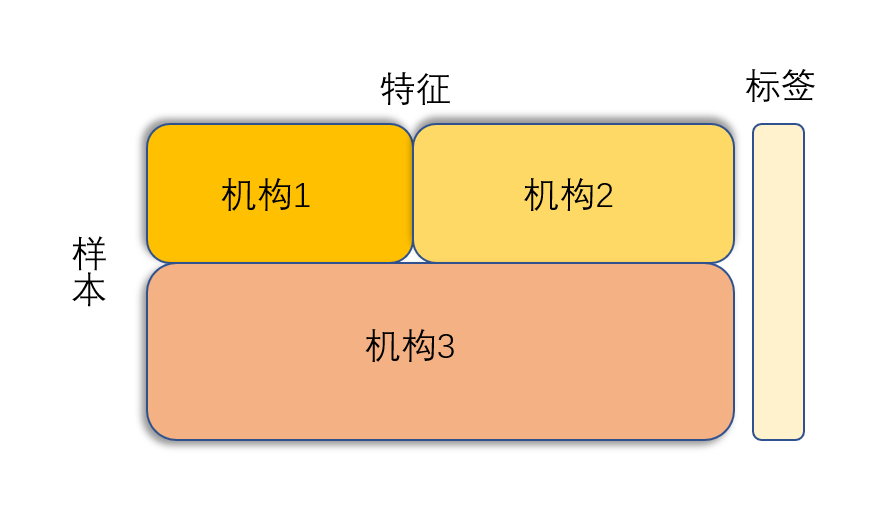
\includegraphics[width=0.5\textwidth]{2D} % requires the graphicx package
	\downcaption{二维问题示意图}
	\label{fig:2D}
\end{figure}

\subsection{二维问题的建立}
\subsubsection{符号与框架}\label{symbol_frame}
基于上述问题的背景,结合Shapley value对数据定价的良好性质,我们依旧希望在Shapley value的基本框架下进行数据价值的分配。而第一部分所针对的数据定价问题是根据样本进行的,也就是所谓的一维问题。而现在我们需要考虑的是对于某些样本的某些特征进行价值分配的问题,简单来说,也就是对于单个样本的单个特征,我们是否有相应的公式进行计算的问题,也就是所谓的二维问题。

首先需要更新一些符号。

定义$N=\{1,2,...n\}$为训练集中的全体样本,$M=\{1,2,...m\}$为数据集中的全体特征。仿照\ref{two maps}节,定义game $\Delta: 2^{N\times M} \rightarrow R$, 特别地, $\Delta(\emptyset, \cdot)=\Delta(\cdot, \emptyset)=0$,
$\varphi: G \rightarrow R^{n\times m}$, G代表上述定义的所有可能的 $\Delta$.
$\varphi_{ij}(\Delta)$ 是第$i$个样本在第$j$个特征下,按照game $\Delta$ 下分配的价值。

仿照\ref{I}节,我们更新$I$的形式如下:
首先定义互动$I$:
\begin{equation}\label{1}
	\Delta(S, F)=\sum_{\substack{W_1\subseteq S, W_2\subseteq F}}I(W_1, W_2), \ \ S\subseteq N, F\subseteq M.
\end{equation}
整理一下:
\begin{equation}
	I(S, F)=\Delta(S, F)-\sum_{W_1\subset S}I(W_1, F)-\sum_{W_2\subset F}I(S, W_2)-\sum_{\substack{W_1\subset S\\ W_2\subset F}}I(W_1, W_2)
	\label{condition}
\end{equation}
再将各互动值按照集合的模来均分:
\begin{equation}\label{2}
	\varphi_{ij}=\sum_{\substack{W_1\subseteq N\backslash\{i\}\\ W_2\subseteq M\backslash\{j\}}}\frac{I(W_1\cup\{i\}, W_2\cup\{j\})}
	{|W_1\cup\{i\}||W_2\cup\{j\}|}
\end{equation}
我们可以证明下面一个定理:
\begin{theorem}\label{thm3}
	上述定义的$\left\langle N, M, \Delta\right\rangle$在公式(\ref{1}),(\ref{condition}),(\ref{2})下的$\varphi_{ij}$形式为:
	\begin{align}
		\label{Shapley Value}
		\varphi_{ij}&=C\sum_{\substack{W_1\subseteq N\backslash\{i\}\\W_2\subseteq M\backslash\{j\}}}
		\frac{[\Delta(W_1\cup\{i\}, W_2\cup\{j\})+
			\Delta(W_1,W_2)-\Delta(W_1\cup\{i\}, W_2)-\Delta(W_1, W_2\cup\{j\})]}{\tbinom{|N|-1}{|W_1|}\tbinom{|M|-1}{|W_2|}}
	\end{align}
\end{theorem}

\subsubsection{定理\ref{thm3}的证明}
我们首先给出一个引理:
\begin{lemma}\label{1d}
	\begin{equation}
		\sum_{\substack{W'\subseteq W\subset S}}(-1)^{|W|-|W'|}\Delta(W')
		=-\sum_{\substack{W'\subset S}}(-1)^{|S|-|W'|}\Delta(W')
	\end{equation}
\end{lemma}
\textbf{证明}

固定$W'$并考虑$W$的选择. $\Delta(W')$的系数$A_{W'}$为:
$$A_{W'}=(-1)^0\tbinom{|S|-|W'|}{0}+(-1)^1\tbinom{|S|-|W'|}{1}+\dots+(-1)^{|S|-|W'|-1}\tbinom{|S|-|W'|}{|S|-|W'|-1}$$
根据二项式定理, 
$$(1-1)^{|S|-|W'|}=0=A_{W'}+(-1)^{|S|-|W'|}$$
$$A_{W'}=-(-1)^{|S|-|W'|}$$
因此,
$$\sum_{\substack{W'\subseteq W\subset S}}(-1)^{|W|-|W'|}\Delta(W')=\sum_{\substack{W'\subset S}}A_{W'}\Delta(W')=
-\sum_{\substack{W'\subset S}}(-1)^{|S|-|W'|}\Delta(W')$$

$\hfill\blacksquare$

对于二维条件下的引理\ref{1d},我们有
\begin{lemma}\label{2d}
	\begin{equation}
		\sum_{\substack{W_1'\subseteq W_1\subset S\\W_2'\subseteq W_2\subset F}}(-1)^{|W_1|+|W_2|-|W_1'|-|W_2'|}\Delta(W_1',W_2')
		=\sum_{\substack{W_1'\subset S\\W_2'\subset F}}(-1)^{|S|+|F|-|W_1'|-|W_2'|}\Delta(W_1',W_2')
	\end{equation}
\end{lemma}

\textbf{证明}

分别对$\Delta(W_1', W_2')$的两变量利用引理\ref{1d}.

$\hfill\blacksquare$

进一步,我们有:
\begin{lemma}
	利用公式(\ref{condition}), 我们有:
	\label{lemma_induct}
	\begin{equation}
		I(S,F)=\sum_{\substack{W_1\subseteq S\\ W_2\subseteq F}}(-1)^{|S|+|F|-|W_1|-|W_2|}\Delta(W_1,W_2)\label{induction}
	\end{equation}
\end{lemma}

\textbf{证明}

证明之前,我们首先看一下如何得到公式(\ref{condition}).
\begin{align*}
	\Delta(S, F)&=\sum_{\substack{W_1\subseteq S\\W_2\subseteq F}}I(W_1, W_2)\\
	&=(\sum_{\substack{W_1=S\\W_2\subseteq F}}+\sum_{\substack{W_1\subset S\\W_2\subseteq F}})I(W_1,W_2)\\
	&=\sum_{W_2\subseteq F}I(S,W_2)+\sum_{\substack{W_1\subset S\\W_2\subseteq F}}I(W_1,W_2)\\
	&=I(S,F)+\sum_{W_2\subset F}I(S,W_2)+\sum_{W_1\subset S}I(W_1,F)+\sum_{\substack{W_1\subset S\\W_2\subset F}}I(W_1,W_2)
\end{align*}

因此我们得到公式(\ref{condition}):
$$I(S, F)=\Delta(S, F)-\sum_{W_1\subset S}I(W_1, W_2)-\sum_{W_2\subset F}I(W_1, W_2)-\sum_{\substack{W_1\subset S\\ W_2\subset F}}I(W_1, W_2)$$

接下来进行数学归纳法:

1、当$|S|\geq 1, |F|=1$, 由公式(\ref{condition}),
$$I(S,F)=\Delta(S,F)-\sum_{W_1\subset S}I(W_1,F)$$
这是一个一维递归形式. 根据论文\cite[6--7]{strumbelj2010efficient}的结论, 我们有:
$$I(S,F)=\sum_{W_1\subseteq S}(-1)^{|S|-|W_1|}\Delta(W_1,F)$$
这满足公式(\ref{induction}). $|S|=1, |F|\geq1$ 同上.

2、假设 $|S|=s, |F|=f$ 并且对于 $A\times B \subset S\times F$ (特别地, $S\times B$ 和 $A\times F$ 也是子集),有下面的等式成立:
\begin{equation}
	I(A,B)=\sum_{\substack{W_1\subseteq A\\ W_2\subseteq B}}(-1)^{|A|+|B|-|W_1|-|W_2|}\Delta(W_1,W_2)
\end{equation}
因此, 由公式(\ref{condition}),
\begin{align*}
	I(S, F)&=\Delta(S, F)-\sum_{W_1\subset S}I(W_1, F)-\sum_{W_2\subset F}I(S, W_2)-\sum_{\substack{W_1\subset S\\ W_2\subset F}}I(W_1, W_2)\\
	&=\Delta(S,F)-\sum_{W_1\subset S}\sum_{\substack{W_1'\subseteq W_1\\W_2'\subseteq F}}(-1)^{|W_1|+|F|-|W_1'|-|W_2'|}
	\Delta(W_1',W_2')\\
	&-\sum_{W_2\subset F}\sum_{\substack{W_1'\subseteq W_1\\W_2'\subseteq W_2}}(-1)^{|S|+|W_2|-|W_1'|-|W_2'|}
	\Delta(W_1',W_2')\\
	&-\sum_{\substack{W_1\subset S\\W_2\subset F}}\sum_{\substack{W_1'\subseteq W_1\\W_2'\subseteq W_2}}(-1)^{|W_1|+|W_2|-|W_1'|-|W_2'|}\Delta(W_1',W_2')\\
	&=\Delta(S,F)+\sum_{\substack{W_1'\subset S\\W_2'\subseteq F}}(-1)^{|S|+|F|-|W_1'|-|W_2'|}\Delta(W_1',W_2')	\\
	&+\sum_{\substack{W_1'\subseteq S\\W_2'\subset F}}(-1)^{|S|+|F|-|W_1'|-|W_2'|}\Delta(W_1',W_2')\\
	&-\sum_{\substack{W_1'\subset S\\W_2'\subset F}}(-1)^{|S|+|F|-|W_1'|-|W_2'|}\Delta(W_1',W_2')\\
	&=\Delta(S,F)+(\sum_{\substack{W_1'\subset S\\W_2'= F}}+\sum_{\substack{W_1'=S\\W_2'\subset F}}
	+2\sum_{\substack{W_1'\subset S\\W_2'\subset F}}-\sum_{\substack{W_1'\subset S\\W_2'\subset F}})(-1)^{|S|+|F|-|W_1'|-|W_2'|}\Delta(W_1',W_2')\\
	&=(\sum_{\substack{W_1'=S\\W_2'= F}}+\sum_{\substack{W_1'\subset S\\W_2'= F}}+\sum_{\substack{W_1'=S\\W_2'\subset F}}
	+\sum_{\substack{W_1'\subset S\\W_2'\subset F}})(-1)^{|S|+|F|-|W_1'|-|W_2'|}\Delta(W_1',W_2')\\
	&=\sum_{\substack{W_1'\subseteq S\\W_2'\subseteq F}}(-1)^{|S|+|F|-|W_1'|-|W_2'|}\Delta(W_1',W_2')
\end{align*}

$\hfill\blacksquare$

接下来我们证明定理\ref{thm3}.

\textbf{证明}

由$\varphi_{ij}$的定义以及引理\ref{lemma_induct},我们有:
\begin{align*}
	\varphi_{ij}&=\sum_{\substack{W_1\subseteq N\backslash\{i\}\\W_2\subseteq M\backslash\{j\}}}\frac{1}{|W_1\cup\{i\}||W_2\cup\{j\}|} \sum_{\substack{W_1'\subseteq W_1\cup\{i\}\\W_2'\subseteq W_2\cup\{j\}}}(-1)^{|W_1|+|W_2|-|W_1'|-|W_2'|}\Delta(W_1',W_2')\\
	&=\sum_{W_2\subseteq M\backslash\{j\}}
	\sum_{W_2'\subseteq W_2\cup\{j\}}\frac{(-1)^{|W_2|-|W_2'|}}{|W_2\cup\{j\}|}\{
	\sum_{W_1\subseteq N\backslash\{i\}}
	\sum_{W_1'\subseteq W_1\cup\{i\}}\frac{(-1)^{|W_1|-|W_1'|}\Delta(W_1',W_2')}{|W_1\cup\{i\}|}\}\\
	&=\sum_{W_2\subseteq M\backslash\{j\}}
	\sum_{W_2'\subseteq W_2\cup\{j\}}\frac{(-1)^{|W_2|-|W_2'|}}{|W_2\cup\{j\}|}
	\sum_{W_1\subseteq N\backslash\{i\}}\frac{(n-s-1)!s!}{n!}\Delta(W_1\cup \{i\},W_2')-\Delta(W_1,W_2')\\
	&=\sum_{W_1\subseteq N\backslash\{i\}}\frac{(n-s-1)!s!}{n!}
	\{\sum_{W_2\subseteq M\backslash\{j\}}
	\sum_{W_2'\subseteq W_2\cup\{j\}}\frac{(-1)^{|W_2|-|W_2'|}}{|W_2\cup\{j\}|}\Delta(W_1\cup \{i\},W_2')-\Delta(W_1,W_2')\}\\
	&=\sum_{W_1\subseteq N\backslash\{i\}}\frac{(n-s-1)!s!}{n!}
	\sum_{W_2\subseteq M\backslash\{j\}}\frac{(m-f-1)!f!}{m!}[\Delta(W_1\cup\{i\}, W_2\cup\{j\})
	+\Delta(W_1,W_2)\\
	&-\Delta(W_1\cup\{i\}, W_2)-\Delta(W_1, W_2\cup\{j\})]\\
	&=\sum_{\substack{W_1\subseteq N\backslash\{i\}\\W_2\subseteq M\backslash\{j\}}}\frac{(n-s-1)!s!}{n!}\frac{(m-f-1)!f!}{m!}[\Delta(W_1\cup\{i\}, W_2\cup\{j\})\\
	&+\Delta(W_1,W_2)-\Delta(W_1\cup\{i\}, W_2)-\Delta(W_1, W_2\cup\{j\})]
\end{align*}


第三和第五个等号来自于一维结果,在第四个等号,我们定义了一个新的
game (我们并不关心$W_1$)$$\Delta'(W_2'):=\Delta(W_1\cup \{i\},W_2')-\Delta(W_1,W_2')$$然后我们再利用一维结果得证.

$\hfill\blacksquare$

\subsection{二维条件下Shapley value的公理化框架}
事实上,我们在上一部分只是根据二维情况下的互动$I$证明了一个价值分配的公式(\ref{Shapley Value})。这一部分我们将从公理化的角度去说明公式(\ref{Shapley Value})是满足公平性分配等一系列公理化条件的唯一分配方式。

\subsubsection{两个映射}
\ref{symbol_frame}节已定义。

\subsubsection{三条公理}
与\ref{three_axioms}节类似,我们先引入三个概念:

1. (Carrier) 称$(S,F)$为$\nu$的一个$\emph{carrier}$,如果

$\nu(W_1, W_2)=\nu(S\cap W_1, F\cap W_2)$,  $\forall W_1 \subset N, W_2 \subset M$. 


2. (Permutation) 如果$\pi_1: N\rightarrow N$是$N$的一个排列, $\pi_2: M\rightarrow M$是$M$的一个排列, 那么$\pi_1\nu$定义为:

$\pi_1^\nu(W_1, F) = \nu(\pi_1(W_1), F)$, $\forall W_1 \subset N$与固定的$F$.

$\pi_2\nu$定义为: 

$\pi_2^\nu(S, W_2) = \nu(\pi_2(S, W_2))$, $\forall W_2 \subset M$与固定的$S$.

3. (Addition) 定义两个game的求和$\nu_1+\nu_2$为:

$(\nu_1+\nu_2)(S, F) = \nu_1(S, F)+\nu_2(S, F)$, $\forall S \subset N, F \subset M$.

公理化条件为:

$S_1$. 如果$(S,F)$是$\nu$的一个carrier, 那么: 

$$\sum_{\substack{i \in S\\j \in M}} \varphi_{ij}(\nu) = \nu(S, M)$$

$$\sum_{\substack{i \in N\\j \in F}} \varphi_{ij}(\nu) = \nu(N, F)$$.


$S_2$. 对于任意的排列$\pi$和$i \in N$,

$$\varphi_{\pi_1(i), \pi_2(j)}(\pi_2(\pi_2\nu)) = \varphi_{ij}(\nu)$$.

$S_3$. 如果$\nu_1$ and $\nu_2$是任意两个game, 那么:

$$\varphi(\nu_1+\nu_2) = \varphi(\nu_1)+\varphi(\nu_2)$$.

\subsubsection{唯一性}
基于上述公理化框架,我们有如下定理:
\begin{theorem}
	满足上述三条公理$S_1, S_2, S_3$的函数$\varphi$存在且唯一,并且满足公式(\ref{Shapley Value}).
	\label{2D_unique}
\end{theorem}
接下来我们证明定理\ref{2D_unique}.

\textbf{证明}

对任意$(S,F)$, 定义一个game $\nu_{S,F,c}$如下:
\begin{equation}
	\nu_{S,F,c}(W_1, W_2)=\left\{
	\begin{array}{lr}
		c, if \ S\subset W_1, F\subset W_2\\
		0, otherwise  
	\end{array}
	\right.
\end{equation}

那么$(S,F)$和它的父集是$\nu$的一个carrier. 因此由$S_1$, 我们有

$$\sum_{\substack{i \in S\\j\in M}} \varphi_{ij}(\nu_{S,F,c}) = \nu_{S,F,c}(S, M) = c$$,
$$\sum_{\substack{i \in N\\j\in F}} \varphi_{ij}(\nu_{S,F,c}) = \nu_{S,F,c}(N, F) = c$$

并且
$$\sum_{\substack{i \in S\cup\{i'\}\\j\in M}} \varphi_{ij}(\nu_{S,F,c}) = c$$, 
$$\sum_{\substack{i \in N\\j\in F\cup\{j'\}}} \varphi_{ij}(\nu_{S,F,c}) = c$$

其中$i' \notin S, j' \notin F$.

因此我们知道,当 $i'\notin S$, $\varphi_{i'j}(\nu_{S,F,c}) = 0$; 当$j'\notin F$, $\varphi_{ij'}(\nu_{S,F,c}) = 0$. 下面我们定义 $\pi_1$为交换$S$中第$i$个与第$j$个元素,其余不变的排列, $\pi_2$为交换$F$中第$i$个与第$j$个元素,其余不变的排列.容易看出 
$\pi_i^{\nu_{S,F,c}}$与$\nu_{S,F,c}$是相同的,对于$i=1, 2$ (因为上述排列并不影响集合之间的包含关系). 因此由$S_2$, 我们有: 

$$\varphi_{i_1j}(\nu_{S,F,c}) = \varphi_{i_2j}(\nu_{S,F,c}), \ \ \forall i_1, i_2 \in S, j \in M$$.
$$\varphi_{ij_1}(\nu_{S,F,c}) = \varphi_{ij_2}(\nu_{S,F,c}), \ \ \forall j_1, j_2 \in F, i \in N$$.

至此我们看到$\varphi$是唯一的, 并且形式为: 
\begin{equation}
	\varphi_{ij}(\nu_{S,F,c})=\left\{
	\begin{array}{lr}
		c/|S||F|, if\ i \in S, j \in F\\
		0, otherwise
	\end{array}
	\right.
\end{equation}
现在定义另一个game $\nu'_{S,F,c}$:
\begin{equation}
	\nu'_{S,F,c}(W_1, W_2)=\left\{
	\begin{array}{lr}
		c, if \ S=W_1, F=W_2\\
		0, otherwise 
	\end{array}
	\right.
\end{equation}
因此对任意$\nu$, 

$$\nu = \sum_{\substack{\emptyset\neq S\subset N\\\emptyset\neq F\subset M}}\nu'_{S,F,\nu(S,F)}$$ 并且由$S_3$,

$$\varphi(\nu) = \sum_{\substack{\emptyset\neq S\subset N\\\emptyset\neq F\subset M}}\varphi(\nu'_{S,F,\nu(S,F)})$$

如果我们可以证明$\varphi(\nu'_{S,F,\nu(S,F)})$的唯一性, 那么$\varphi(\nu)$就是唯一的.
我们利用数学归纳法来证明.

假设当$|S| = p + 1 ..... n, |F| = q + 1 ..... m$, $\varphi(\nu'_{S,F,c})$是唯一的. (对于 
$|S| = n, |F| = m$很显然,因为$\varphi(\nu'_{N,M,c})$ = $\varphi(\nu_{N,M,c})$).
我们将证明当$p\leq|S|\leq p+1, q\leq|F|\leq q+1$, $\varphi(\nu'_{S,F,c})$也是唯一的.
例如, 我们证明$|S|=p, |F|=q$下的情形.

记$S_1, ....., S_l$为$S$所有可能的父集, $F_1, ....., F_r$为$F$所有可能的父集.
那么,

$$\nu_{S,F,c} = \nu'_{S,F,c}+\sum_{i=1}^{l}\sum_{j=1}^{r}\nu'_{S_i,F_j,c}$$

因此由$S_3$,
\begin{equation}
	\varphi(\nu_{S,F,c}) = \varphi(\nu'_{S,F,c})+\sum_{i=1}^{l}\sum_{j=1}^{r}\varphi(\nu'_{S_i,F_j,c})\label{11}
\end{equation}


因为除了$\varphi(\nu'_{S,F,c})$之外,其余各项均是唯一的, $\varphi(\nu'_{S,F,c})$当然也是唯一确定的.

接下来我们继续探索$\varphi(\nu'_{S,F,c})$的形式.

假设 
\begin{equation}
	\label{111}
	\varphi_{ij}(\nu'_{S,F,c})=\left\{
	\begin{array}{lr}
		\frac{(s-1)!(n-s)!}{n!}\frac{(f-1)!(m-f)!}{m!}\cdot c, if\  i\in S, j\in F \\
		\frac{s}{n-s}\frac{(s-1)!(n-s)!}{n!}\frac{f}{m-f}\frac{(f-1)!(m-f)!}{m!}\cdot c, if\  i\notin S, j\notin F \\ 
		-\frac{(s-1)!(n-s)!}{n!}\frac{f}{m-f}\frac{(f-1)!(m-f)!}{m!}\cdot c, if\  i\in S, j\notin F \\ 
		-\frac{s}{n-s}\frac{(s-1)!(n-s)!}{n!}\frac{(f-1)!(m-f)!}{m!}\cdot c, if\  i\notin S, j\in F
	\end{array}
	\right.
\end{equation}


其中$s = |S| = p+1 ,......, n, f = |F| = q+1 ,......, m$.

利用公式(\ref{11}), 我们可以证明在$|S| = k$时,公式(\ref{111})也成立.

最后通过
\begin{align*}
	\varphi(\nu) &= \sum_{\substack{\emptyset\neq S\subset N\\\emptyset\neq F\subset M}}\varphi(\nu'_{S,F,\nu(S,F)})\\
	&=\sum_{\substack{\emptyset\neq S_i^+\subset N\\\emptyset\neq F_j^+\subset M}}\varphi(\nu'_{S_i^+,F_j^+,\nu(S_i^+,F_j^+)})
	+\sum_{\substack{\emptyset\neq S_i^-\subset N\\\emptyset\neq F_j^-\subset M}}\varphi(\nu'_{S_i^-,F_j^-,\nu(S_i^-,F_j^-)})\\
	&+\sum_{\substack{\emptyset\neq S_i^+\subset N\\\emptyset\neq F_j^-\subset M}}\varphi(\nu'_{S_i^+,F_j^-,\nu(S_i^+,F_j^-)})
	+\sum_{\substack{\emptyset\neq S_i^-\subset N\\\emptyset\neq F_j^+\subset M}}\varphi(\nu'_{S_i^-,F_j^+,\nu(S_i^-,F_j^+)})
\end{align*}
其中我们定义$S_i^+ = \{\emptyset\neq S\subset N| i\in S\}$, $S_i^- = S_i^+-\{i\}$, $F_j^+ = \{\emptyset\neq F\subset M| j\in F\}$ , $F_j^- = F_j^+-\{j\}$.

进而($s=|S_i^+|=|S|$, $f = |F_j^+|=|F|$)
\begin{equation}
	\begin{aligned}
		\varphi_{ij}(\nu) &= \sum_{\substack{\emptyset\neq S_i^+\subset N\\\emptyset\neq F_j^+\subset M}}
		\{\frac{(s-1)!(n-s)!}{n!}\frac{(f-1)!(m-f)!}{m!}\cdot \nu(S_i^+, F_j^+)\\
		&+\frac{s-1}{n-(s-1)}\cdot\frac{(s-1-1)!(n-(s-1))!}{n!}\frac{f-1}{m-(f-1)}\\
		&\cdot\frac{(f-1-1)!(m-(f-1))!}{m!}
		\cdot\nu(S_i^+-\{i\}, F_j^+-\{j\})\\
		&-\frac{(s-1)!(n-s)!}{n!}\frac{f-1}{m-(f-1)}\cdot\frac{(f-1-1)!(m-(f-1))!}{m!}\cdot\nu(S_i^+, F_j^+-\{j\})\\
		&-\frac{s-1}{n-(s-1)}\cdot\frac{(s-1-1)!(n-(s-1))!}{n!}\frac{(f-1)!(m-f)!}{m!}\cdot \nu(S_i^+-\{i\}, F_j^+)\}\\
		&=\sum_{\substack{i\in S\subset N\\j\in F\subset M}}
		\frac{(s-1)!(n-s)!}{n!}\frac{(f-1)!(m-f)!}{m!}\cdot \{\nu(S, F)+\nu(S-\{i\}, F-\{j\})\\
		&-\nu(S, F-\{j\})-\nu(S-\{i\}, F)\}
	\end{aligned}
\end{equation}

$\hfill\blacksquare$

\subsection{算法}
令$\Pi_1$为$S$中的所有$s!$个排列的均匀分布, $\Pi_2$分别为$F$中的所有$f!$个排列的均匀分布。
基于公式(\ref{Shapley Value}),令常数$C=1/|N||M|$, 我们可以得到其等价的期望形式:
\begin{equation}
	\varphi_{ij}=\mathbb{E}_{\substack{\pi_1\sim\Pi_1\\\pi_2\sim\Pi_2}}[\Delta(S_{\pi_1}^i\cup\{i\}, F_{\pi_2}^j\cup\{j\})
	+\Delta(S_{\pi_1}^i,F_{\pi_2}^j)-\Delta(S_{\pi_1}^i\cup\{i\}, F_{\pi_2}^j)-\Delta(S_{\pi_1}^i, F_{\pi_2}^j\cup\{j\})]
\end{equation}
其中$S_{\pi_1}^i$表示在排列$\pi_1$下,所有在数据$i$之前出现的数据的集合,$F_{\pi_2}^j$类似定义。($S_{\pi_1}^i=\emptyset$ 如果$i$是第一个元素,$F_{\pi_2}^j=\emptyset$如果$j$是第一个元素。

通过使用蒙特卡洛方法,我们可以得到如下算法:
\begin{algorithm}[H]
	\caption{ Truncated Monte Carlo Shapley} %算法的名字
	\label{alg}
	\hspace*{0.02in} {\bf Input: Train data \textsl{S}=\{1,2, $\dots$, s\}, \textsl{F}=\{1,2, $\dots$, f\}, learning algorithm 
		$\mathcal{A}$, performace score $\Delta$}\\ %算法的输入, \hspace*{0.02in}用来控制位置,同时利用 \\ 进行换行
	\hspace*{0.02in} {\bf Output:} %算法的结果输出
	Shapley value of training points: $\varphi_{ij}$, for $i=1,\dots,s, j=1,\dots,f$
	\begin{algorithmic}[1]
		\State Initialize $\varphi_{ij}$=0 for $i=1,\dots,s, j=1,\dots,f$ and t=0 % \State 后写一般语句
		\While{Convergence criteria not met do} % While语句,需要和EndWhile对应
		\State $t\leftarrow t+1$\\
		$\pi_1^t$:Random permutation of train data points in S\\
		$\pi_2^t$:Random permutation of train data points in F\\
		$\delta_{00}^t, \delta_{10}^t, \delta_{01}^t\leftarrow \Delta(\emptyset,\emptyset, \mathcal{A})$
		\For{$j \in \{1,2, \dots, f\}$} % For 语句,需要和EndFor对应
		\For{$i \in \{1,2, \dots, s\}$}
		\If{$|\Delta(S,F)-\delta_{ij}^t|<$ Perfomace Tolerance} % If 语句,需要和EndIf对应
		\State $\delta_{ij}^t\leftarrow\delta_{i-1,j}^{t}$
		\Else \quad$\delta_{ij}^t\leftarrow \Delta((\pi_1^t[1],\dots,\pi_1^t[i]),(\pi_2^t[1],\dots,\pi_2^t[j]),\mathcal{A})$
		\EndIf 
		\State $\varphi_{\pi_1^t[i]\pi_2^t[j]}\leftarrow \frac{t-1}{t}\varphi_{\pi_1^t[i]\pi_2^t[j]}+\frac{1}{t}(\delta_{ij}^t+
		\delta_{i-1,j-1}^t-\delta_{i,j-1}^t-\delta_{i-1,j}^t)$
		\EndFor 
		\EndFor 
		\EndWhile 
	\end{algorithmic}
\end{algorithm}

\subsection{实验}
针对于算法\ref{alg}的输入,我们将训练数据集选为Iris数据集(包含两类各50个样本),算法选择为Logistic回归(进行二分类问题),表现度量(Performance score)选择为Accuracy(准确度)。表\ref{table Iris}为Iris数据集的概况:
\begin{table}[H]\small
	\centering
	\topcaption{Iris数据集(取其中五行)}
	\label{table Iris}
	\resizebox{\textwidth}{20mm}{
	\begin{tabular}{cccccc}
		\toprule[1.5pt]
		\textbf{Sample} & \textbf{Sepal Length(cm)} & \textbf{Sepal Width(cm)} & \textbf{Petal Length(cm)} 
		& \textbf{Petal Width(cm)} & \textbf{Species} \\
		\midrule[1pt]
		0& 5.1 & 3.5 & 1.4 & 0.2 & Iris-setosa \\
		1& 4.9 & 3.0 & 1.4 & 0.2 & Iris-setosa \\
		2& 4.7 & 3.2 & 1.3 & 0.2 & Iris-setosa \\
		3& 5.7 & 2.8 & 4.5 & 1.3 & Iris-versicolor \\
		4& 6.3 & 3.3 & 4.7 & 1.6 & Iris-versicolor \\
		\bottomrule[1.5pt]
	\end{tabular}}
	
\end{table}
根据算法\ref{alg}计算得到的Shapley value如表\ref{table value}所示:
\begin{table}[H]\small
	\centering
	\topcaption{Iris数据集的Shapley value(取前五行)}
	\label{table value}
	\begin{tabular}{ccccc}
		\toprule[1.5pt]
		\textbf{Sample} & \textbf{Value of feature 1} & \textbf{Value of feature 2} & \textbf{Value of feature 3} 
		& \textbf{Value of feature 4} \\
		\midrule[1pt]
		0&0.00325884 & 0.00417191 & 0.00390889 & 0.00456872 \\
		1&0.00168026 & 0.00631591 & 0.004814   & 0.00575  \\
		2&0.00425511 & 0.00493199 & 0.00474105 & 0.00479602 \\
		3&0.00277849 & 0.00563966 & 0.0057057  & 0.00560915 \\
		4& 0.00309975 & 0.00503531 & 0.00513633 & 0.00529536 \\
		\bottomrule[1.5pt]
	\end{tabular}
	
\end{table}
前三个样本的计算结果的收敛图像如图\ref{fig:convergence}所示:
\begin{figure}[H]
	\centering
	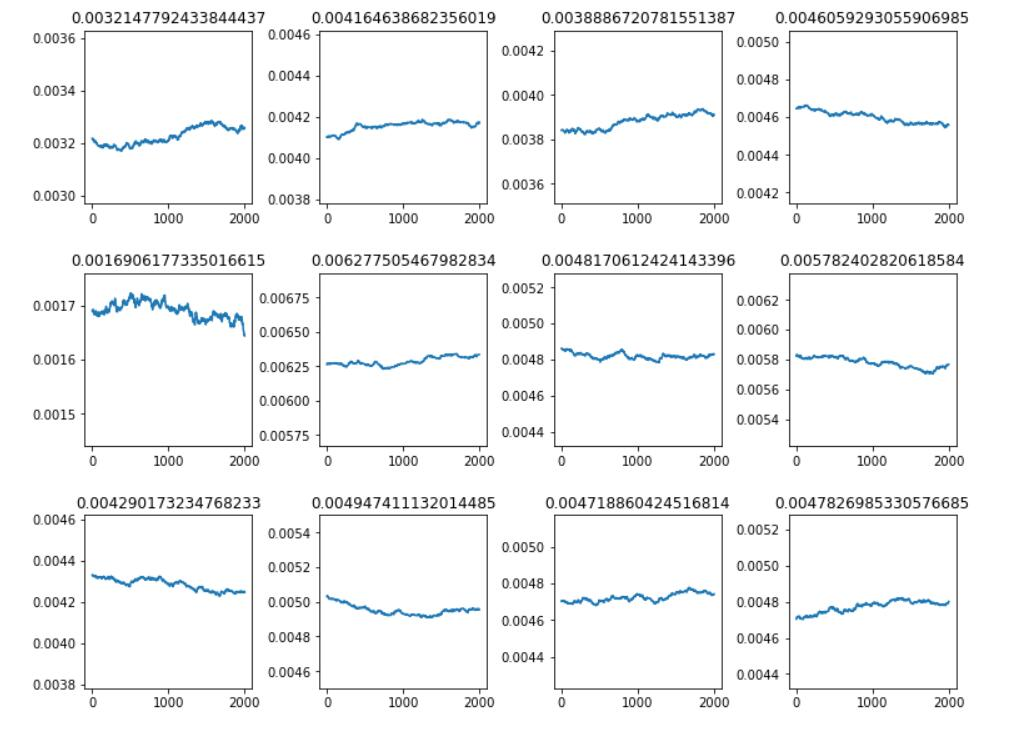
\includegraphics[width=0.5\textwidth]{convergence_plot} % requires the graphicx package
	\downcaption{Shapley value的收敛图像(前三个样本)}
	\label{fig:convergence}
\end{figure}
\section{算法加速}
这里我们考虑一维情形,二维的情形也是容易得到的。

一维情形下的蒙特卡洛算法如下\cite{ghorbani2019data}:
\begin{algorithm}[H]
	\caption{Truncated Monte Carlo Shapley}%算法名字
	\label{alg1}
	\hspace*{0.02in} {\bf Input: Train data \textsl{D}=\{1,2, $\dots$, n\}, learning algorithm $\mathcal{A}$, performace score $V$}\\ %算法的输入, \hspace*{0.02in}用来控制位置,同时利用 \\ 进行换行
	\hspace*{0.02in} {\bf Output:} %算法的结果输出
	Shapley value of training points: $\varphi_{i}$, for $i=1,\dots,n$
	\begin{algorithmic}[1]
		\State Initialize $\varphi_{i}$=0 for $i=1,\dots,n$ and t=0;
		\While{Convergence criteria not met do}
		\State $t\leftarrow t+1$\\
		$\pi^t$:Random permutation of train data points\\
		$v_0^t\leftarrow V(\emptyset,\mathcal{A})$\\
		\For{$j \in \{1,2, \dots, n\}$}
		\If{$|V(D)-v_{j-1}^t|<$ Perfomace Tolerance}
		\State $v_{j}^t\leftarrow v_{j-1}^{t}$
		\Else \quad{$v_{j}^t\leftarrow V((\pi^t[1],\dots,\pi^t[j]),\mathcal{A})$}
		\EndIf
		\State $\varphi_{\pi^t[j]}\leftarrow \frac{t-1}{t}\varphi_{\pi^t[j]}+\frac{1}{t}(v_j^t-v_{j-1}^t)$
		\EndFor
		\EndWhile
	\end{algorithmic}	
	
\end{algorithm}

一方面,一维Shapley value的计算复杂度体现在下式的求和指标上:
$$\varphi_i(\nu) = \sum_{i\in S\subset N}\frac{(s-1)!(n-s)!}{n!}\cdot (\nu(S)-\nu(S-\{i\}), \ \ \nu \in G, s=|S|$$. 
即:我们需要指数级别的检索,这是Shapley value难以计算的根源之一。

另一方面,我们在利用蒙特卡洛方法计算时,在每计算一次边际贡献,都需要进行一次训练以及对Performance的测量,这既耗费时间,又会大大增加计算成本。

为了衡量计算复杂度,定义Shapley value的$(\epsilon, \delta)$估计:
\begin{definition}
	称$\hat{s}$为Shapley value $s \in \mathbb{R}^N$的一个$(\epsilon, \delta)$估计,如果
	$P[||s-\hat{s}||_2\leq \epsilon]\geq \delta$.
\end{definition}
另外,我们以计算Performance的次数(Test number)作为衡量复杂度的指标。
参考论文\cite{jia2019towards},相关算法的计算复杂度如表\ref{table alg}所示:
\begin{table}[H]\small
	\centering
	\topcaption{一维Shapley value各算法复杂度分析}
	\label{table alg}
	\begin{tabular}{ccc}
		\toprule[1.5pt]
		\textbf{算法名称} & \textbf{计算复杂度} & \textbf{误差} \\
		\midrule[1pt]
		Baseline(算法\ref{alg1})& $\mathcal{O}(N^2\log N)$ & $(\epsilon, \delta)$估计  \\
		Group Testing & $\mathcal{O}(N(\log N)^2)$ & $(\epsilon, \delta)$估计  \\
		Compressive Permutation Sampling&$\mathcal{O}(N\log(\log N))$ & $||s-\hat{s}||_2\leq C_{1,K}\epsilon+C_{2,K}\frac{\sigma_K(s)}{\sqrt{K}}$ \\
		\bottomrule[1.5pt]
	\end{tabular}
	
\end{table}
其中$C_{1,K}, C_{2,K}$为关于$K$的常数,$K$与$\sigma_K(s)$为表示Shapley value稀疏性的一些度量。
\






\section{结论与展望}
本文主要根据一维Shapley value的公理化框架与推导过程,结合数据价值分配的现实场景,提出了二维Shapley value的公理化框架及相应形式,并利用其进行计算,实验结果收敛并符合预期。

未来在Shapley value框架下可以进行一系列工作,如:减小方差、如何选择测试集来恰当的衡量Performance以及如何构造Shapley value的置信区间等。这些问题也是将Shapley value推向现实应用场景必不可少的工作。

而在二维应用场景下,我们还会遇到数据不完整以及标签标注贡献计算的问题,这些问题也需要进一步思考与完善。
\backmatter 


\bibliography{sample}
\appendixs{}%附录,直接在后面加内容
\lstinputlisting[
style       =   Python,
caption     =   {\bf 代码},
label       =   {DShap.py}
]{DShap.py}

\begin{acknowledgment}%致谢
经过四个多月的学习和工作,我完成了这次毕设。从开始接到论文题目到阅读论文与代码,再到定理的证明与推导,代码的调试与实验的进行,每一步对我来说都是新的尝试与挑战,也让我学到了很多知识与技能,更让我找到了科研的兴趣与热情。

在这个过程中,我要感谢武师姐帮助我检查证明过程的错误,志凯师兄帮助我学会利用Jupyterlab等平台以及帮我调试代码,还要感谢我的指导老师常象宇老师对我的指导与鼓励,另外还有其他的一些老师和同学也给了我很多帮助,在此一并谢过,感谢大家!


\end{acknowledgment}


\end{document}  